\documentclass{standalone}
\usepackage{tikz} % Import the tikz package
\usetikzlibrary{automata} % Import library for drawing automata
\usetikzlibrary{positioning} % ...positioning nodes
\usetikzlibrary{arrows} % ...customizing arrows
\tikzset{node distance=2.5cm,
    every state/.style={
        semithick,
        fill=gray!10},
    initial text={},
    double distance=2pt,
    every edge/.style={
        draw,
        ->,>=stealth',
        auto,
        semithick}}
\let\epsilon\varepsilon
\begin{document}
    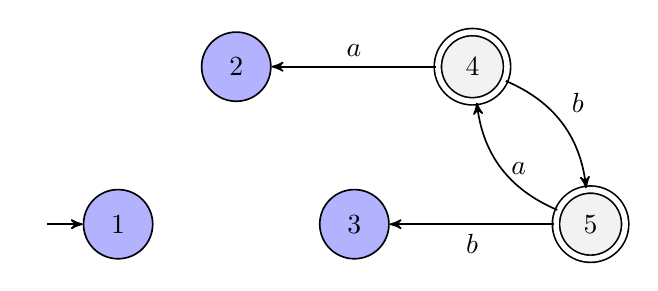
\begin{tikzpicture}
        \node[initial,state,fill=blue!30!white] (1) at (-3,0) {$1$};
        \node[state,fill=blue!30!white] (2) at (-1.5,2) {$2$};
        \node[state,fill=blue!30!white] (3) at (0,0) {$3$};
        \node[state,accepting] (4) at (1.5,2) {$4$};
        \node[state,accepting] (5) at (3,0) {$5$};

        % \draw (1) edge[bend right] node {$a$} (2);
        % \draw (1) edge[below] node {$b$} (3);

        % \draw (2) edge[bend right,left] node {$a$} (1);
        % \draw (2) edge[bend left,left] node {$b$} (3);

        % \draw (3) edge[bend left,left] node {$a$} (2);
        % \draw (3) edge[loop below] node {$b$} (3);

        \draw (4) edge[above] node {$a$} (2);
        \draw (4) edge[bend left] node {$b$} (5);

        \draw (5) edge[bend left,right] node {$a$} (4);
        \draw (5) edge[below] node {$b$} (3);
    \end{tikzpicture}
\end{document}